\section
[$G/G/1$  and $G/G/c$ Queue: Approximations]
{$\mathbf{G/G/1}$  and $\mathbf{G/G/c}$ Queue: Approximations}
\label{sec:gg1}

In manufacturing settings it is quite often the case that the arrival
process at a station is not Poisson. For instance, if processing times
at a station are nearly constant, and the jobs of this station are
sent to a second station for further processing, the inter-arrival
times at the second station must be more or less equal. Hence, in this
case, the SCV of the arrivals at the second station $C_{a,2}^2$ is
most probably smaller than 1. As a consequence the
Pollackzek-Khintchine formula for the $M/G/1$-queue can no longer be
reliably used to compute the average waiting times.  As a second,
trivial case, if the inter-arrival times of jobs are 1 hour always and
service times 59 minutes always, there simply cannot be queue. Thus,
the $M/G/1$ waiting time formula cannot, and should not, be applied to
approximate the average waiting time of the $G/G/1$ queue. 

There is no formula as yet by which the average waiting times for the
$G/G/1$ queue can be computed; only approximations are available. One
such simple and robust approximation is based on the following
observation. Recall  the waiting time in queue for the $M/M/1$ queue:
\begin{equation*}
  \E{W_Q(M/M/1)} = \frac{\rho}{1-\rho} \E S = 
\frac{1_a + 1_b}2 \frac{\rho}{1-\rho} \E S,
\end{equation*}
where we label the number $1$ with $a$ and $b$. When generalizing this
result to the $M/G/1$ queue we get
\begin{equation*}
  \E{W_Q(M/G/1)} = \frac{1_a + C_s^2}2 \frac{\rho}{1-\rho} \E S,
\end{equation*}
Thus, $1_b$ in the expression for the $M/M/1$ queue is replaced by
$C_s^2$ in the expression for the $M/G/1$ queue. As a second
generalization, Kingman proposed to replace $1_a$ in this formula by
the SCV of the inter-arrival times
\begin{equation*}
C_a^2 = \frac{\V X}{(\E X)^2}
\end{equation*}
resulting in
\begin{equation*}
  \E{W_Q(G/G/1)} \approx \frac{C_a^2 + C_s^2}2 \frac{\rho}{1-\rho} \E S.
\end{equation*}

This formula is reasonable accurate; for more, related, expressions we
refer to \citet{bolch06:_queuein_networ_markov_chain} and
\citet{hall91:_queuein_method_servic_manuf}. With Little's law we can
compute $\E{L_Q}$ from the above. Moreover, $\E W = \E{W_Q} + \E S$,
and so on.


It is crucial to memorize the \emph{scaling} relations that can be
seen from the $G/G/1$ waiting time formula. Roughly:
\begin{enumerate}
\item $\E{W_Q} \sim (1-\rho)^{-1}$. The consequence is that the waiting
  time increases \emph{very steeply} when~$\rho$ is large, hence is
  very sensitive to the actual value of $\rho$ when $\rho$ is large.
\item $\E{W_Q} \sim C_a^2$ and $\E{W_Q} \sim C_s^2$. Hence, reductions
  of the variation of the inter-arrival and service times do affect the
  waiting time, but only linearly.
\item $\E{W_Q} \sim \E S$. Thus, working in smaller job sizes reduces
  the waiting time also. The average queue length does not decrease by
  working with smaller batches, but jobs are more `uniformly spread'
  over the queue. This effect lies behind the idea to do
  `lot-splitting', i.e., rather than process large jobs, split jobs
  into multiple small jobs (assuming that setup times are negligible),
  so that the waiting time per job can be reduced.
\end{enumerate}

These insights prove very useful when trying to reduce waiting times
in any practical situation. First try to reduce the load (by blocking
demand or increasing the capacity), then try to reduce the variability
(e.g., by planning the arrival times of jobs), and finally, attempt to
split jobs into multiple smaller jobs and use the resulting freedom to
reschedule jobs in the queue.

For the $G/G/c$ queue we also only have an approximation: 
\begin{equation}\label{eq:7}
  \E{W_Q} = \frac{C_a^2+C_e^2}2 \frac{\rho^{\sqrt{2(c+1)}-1}}{c(1-\rho)} \E S.
\end{equation}

Even though the above results are only approximate, they prove to be
exceedingly useful when designing queueing systems and analyzing the
effect of certain changes, in particular  changes in capacity,
variability and service times.

Clearly, Kingman's equation requires an estimate of the SCV $C_a^2$ of
the inter-arrival times and the SCV $C_s^2$ of the service times. Now,
as already mentioned in Section~\ref{sec:discrete-time-case}, it is
not always easy in practice to determine the actual service time
distribution, one reason being that service times are often only
estimated by a planner, but not actually measured. Similarly, the
actual arrival moments of jobs are often not registered, mostly just
the date or the hour, perhaps, that a customer arrived.  Hence, it is
often not possible to estimate $C_a^2$ and $C_s^2$ from information
that is available.  However, when for instance the number of arrivals
per day have been logged for some time, i.e., we know
$\{a_n, n=1,\ldots, N\}$ for some $N$, we can this information instead
of the the inter-arrival times $\{X_k\}$, to obtain insight into the
relevant SCVs.  Here we present a relation to compute $C_a^2$ from
$\{a_n\}$; of course it can be applied to $C_s^2$ as well.

\begin{theorem} The SCV of the inter-arrival times can be estimated
  with the following formula
\begin{equation*}
C_a^2 \approx \frac{\tilde \sigma^2}{\tilde \lambda},
\end{equation*}
where 
\begin{equation*}
\tilde  \lambda = \lim_{n\to\infty} n^{-1} \sum_{i=1}^n a_i,\quad  
\tilde  \sigma^2 = \lim_{n\to\infty} n^{-1} \sum_{i=1}^n a_i^2 - \tilde \lambda^2,
\end{equation*}
in words, $\tilde \lambda$ is the average number of arrivals per
period, e.g., per day, and $\tilde \sigma^2 $ is the variance of the
number of arrivals per period.
\end{theorem}

\begin{proof}
  The proof is based on an argument in \cite{cox62:_renew_theor}. We
  use quite a bit of the notation developed in
  Section~\ref{sec:rate-stability}. Let $\{A(t), t\geq 0\}$ be the
  number of arrivals that occur up to (and including) time $t$. We
  assume that $\{A(t)\}$ is a renewal process such that the
  inter-arrival times $\{X_k, k=1, 2, \ldots\}$ with
  $X_k = A_{k}-A_{k-1}$, are i.i.d. with mean $1/\lambda$ and standard
  deviation~$\sigma$. (Observe that $\sigma$ is not the same as
  $\tilde \sigma$ above.) Note that $C_a^2$ is defined in terms of
  $\lambda$ and $\sigma$ as:
\begin{equation*}
C_a^2 = \frac{\V{X_i}}{(\E{X_i})^2} = \frac{\sigma^2}{1/\lambda^2} = \lambda^2 \sigma^2.
\end{equation*}

Next, let $A_k$ be the arrival time of the $k$th arrival. The
following useful relation between $A(t)$ and $A_k$ enables us to prove
our result (recall that we uses a similar relation in the derivation
of the Poisson process):
\begin{equation*}
\P{A(t) < k} = \P{A_k > t}
\end{equation*}

Since the inter-arrival times have finite mean and second moment by
assumption, we can apply the central limit law to obtain that, as
$k\to\infty$,
\begin{equation*}
\frac{A_k -k/\lambda}{\sigma \sqrt k} \to N(0,1),
\end{equation*}
where $N(0,1)$ is a standard normal random variable with
distribution $\Phi(\cdot)$.  Similarly,
%
\begin{equation*}
\frac{A(t) -\lambda t}{\alpha \sqrt t} \to N(0,1)
\end{equation*}
for an $\alpha$ that is yet to be determined. Thus,
$\E{A(t)} = \lambda t$ and $\V{A(t)}=\alpha^2 t$.

Using that $\P{N(0,1) \leq y} =
\P{N(0,1) > -y}$ (and $\P{N(0,1)=y} = 0$) we have that
%
\begin{align*}
\Phi(y) &\approx \P{\frac{A_k - k/\lambda}{\sigma \sqrt k }\leq y} \\
        &= \P{\frac{A_k - k/\lambda}{\sigma \sqrt k} >  -y} \\
        &=  \P{A_k >  \frac k\lambda - y \sigma \sqrt k}.
\end{align*}
Define for ease
\begin{equation*}
t_k = \frac{k}\lambda - y \sigma \sqrt k.
\end{equation*}
We can use the above relation between the distributions of~$A(t)$
and~$A_k$ to see that~$\P{A_k >t_k } = \P{A(t_k) <k}$. With this we
get,
\begin{align*}
\Phi(y)
        &\approx  \P{A_k >  t_k } \\
        &=  \P{A(t_k) <  k } \\
        &=  \P{\frac{A(t_k) - \lambda t_k}{\alpha \sqrt{t_k}} < 
\frac{k-\lambda t_k}{\alpha \sqrt{t_k}}}.
\end{align*}
Since, $(A(t_k) - \lambda t_k)/ \alpha \sqrt{t_k} \to N(0,1)$
as $t_k \to \infty$, the above implies that
\begin{equation*}
\frac{k-\lambda t_k}{\alpha \sqrt{t_k}} \to y,
\end{equation*}
as $t_k \to \infty$.  Using the above definition of $t_k$, the left
hand of this equation can be written as
\begin{equation*}
\frac{k-\lambda t_k}{\alpha \sqrt{t_k}} =
\frac{\lambda \sigma \sqrt k }{\alpha \sqrt{k/\lambda + \sigma\sqrt k}} y.
\end{equation*}
Since $t_k \to \infty$ is implied by (and implies)
$k\to\infty$, we therefore want that $\alpha$ is such that
\begin{equation*}
\frac{\lambda \sigma \sqrt k }{\alpha \sqrt{k/\lambda + \sigma\sqrt k}} y \to y,
\end{equation*}
as $k\to\infty$. This is precisely the case when
\begin{equation*}
\alpha = \lambda^{3/2}\sigma.
\end{equation*}
Finally, for $t$ large (or, by the same token $k$ large),
\begin{align*}
\frac{\sigma_k^2}{\lambda_k} &= \frac{\V{A(t)}}{\E{A(t)}} \approx \frac{\alpha^2 t}{\lambda t} 
= \frac{\alpha^2}{\lambda} = \frac{\lambda^3\sigma^2}{\lambda} = \lambda^2 \sigma^2 \\
&= C_a^2,
\end{align*}
where the last equation follows from the above definition of $C_a^2$.  The proof is complete.
\end{proof}



\begin{question}
  Show that~\eqref{eq:7} reduces to the result known for the $M/M/1$ and $M/G/1$ queues. 
    \hint{ Take $c=1$.}
  \begin{solution}
    If $c=1$, as is the case for the $M/M/1$ queue, $\sqrt{2(c+1)} - 1=2-1=1$, so that~\eqref{eq:7} reduces to $\E{W_Q} = \rho/(1-\rho) \E S$. Recall that $C_a^2=C_s^2=1$ for the $M/M/1$. 
  \end{solution}
\end{question}


\begin{question}
  Is Eq.~\eqref{eq:24} also valid for the $G/G/1$ queue? Why (not)?
  \begin{solution}
    Not necessarily. Since jobs do not arrive in general as a Poisson
    process, we cannot use the PASTA property to conclude that the
    time average queue length $\E{L_Q}$ is the same as the average
    queue length as observed by customers.

(Can you provide an example that shows this difference?
    Hint, we did this earlier.)
  \end{solution}
\end{question}



\begin{question}
  Consider a queue $n$ servers, with generally distributed
  inter-arrival times, generally distributed service times, and the
  system can contain at most $K$ customers, i.e, the $G/G/n/K$ queue.
  Let $\lambda$ be the arrival rate, $\mu$ the service rate, $\beta$
  the long-run fraction of customers lost, and $\rho$  the average
  number of busy/occupied servers
  Show that 
  \begin{equation*}
    \beta = 1 - \rho\frac{\mu}{\lambda}.
  \end{equation*}
\begin{solution}
  This follows from the observation that $\lambda(1-\beta)$ is the net
  arrival rate, as jobs are lost at a rate $\lambda\beta$ . Hence, the
  load must be $\lambda(1-\beta)/\mu$. As the load must be equal to
  $\rho$, it follows that $\rho = \lambda(1-\beta)/\mu$, from which the
  other result immediately follows.
\end{solution}
\end{question}

\begin{question}
  \begin{enumerate}
  \item Consider a single-server queue at which every minute a
    customer arrives, precisely at the first second. Each customer
    requires precisely $50$ seconds of service. 
What are $\rho$,
    $\E L$, $C_a^2$, and $C_S^2$?
  \item Consider the same single-server system, but now the customer
    service time is stochastic: with probability $1/2$ a customer
    requires $1$ minute and $20$ seconds of service, and with
    probability $1/2$ the customer requires only $20$ seconds of
    service.  What are $\rho$, $C_a^2$, and $C_S^2$?
  \end{enumerate}
  \begin{solution}
    \begin{enumerate}
    \item $\rho = \lambda \E S = 1/60 \cdot 50 = 5/6$. Since job
      arrivals do not overlap any job service, the number of jobs in
      the system is 1 for $50$ seconds, then the server is idle for 10
      seconds, and so on. Thus $\E L = 1\cdot5/6 = 5/6$. There is no
      variance in the inter-arrival times, and also not in the service
      times, thus $C_a^2 = C_s^2 = 0$. Also $\E{W_Q}=0$ since
      $\E{L_Q}=0$. Interestingly, we get the same from Kingman's formula.
    \item Again $\E S$ is 50 seconds, so that $\rho = 5/6$. Also
      $C_a^2=0$. For the $C_S^2$ we have to do some work. 
      \begin{equation*}
        \begin{split}
          \E S &=  \frac{20}2 + \frac{80}2 = 50 \\
          \E{S^2} &=  \frac{400}2 + \frac{6400} 2 = 3400 \\
          \V S &=  \E S^2 - (\E S)^2 = 3400 - 2500 = 900 \\
          C_S^2 &=  \frac{\V S}{(\E S)^2} = \frac{900}{2500}=\frac{9}{25}.
        \end{split}
      \end{equation*}
    \end{enumerate}
  It is crucial to remember from this exercise that knowledge of the
  utilization is not sufficient to characterize the average queue
  length.
  \end{solution}
\end{question}

\begin{question}
  For the $G/G/1$ queue, prove that the fraction of jobs that see $n$
  jobs in the system is the same as the the fraction of departures that
  leave $n$ jobs behind. What condition have you used to prove this?
%\item Motivate that for  the $G/M/1$, $\delta(n) = p(n)$, i.e.,  departures see time averages. 
  \begin{solution}
    All follows straightaway from the definitions in the main text. In
    the $G/G/1$ queue jobs arrive and depart in single units. Hence,
    $|A(n,t)-D(n,t)|\leq 1$, c.f., Eq.~(\ref{eq:19}). Then, 
    \begin{equation*}
      \frac{A(t)}{t}\frac{A(n,t)}{A(t)} \approx 
      \frac{D(t)}{t}\frac{D(n,t)}{D(t)}. 
    \end{equation*}
    The left hand side goes to $\lambda \pi(n)$ as $t\to\infty$, and
    the right hand side to $\gamma \delta(n)$. Use the fact that we
    always assume, implicitly, that the system is stable, so that
    $\lambda = \gamma$. As a consequence $\delta(n) = \pi(n)$.
  \end{solution}
\end{question}

\begin{question}
  (Hall 5.19) When a bus reaches the end of its line, it undergoes a
  series of inspections. The entire inspection takes 5 minutes on
  average, with a standard deviation of 2 minutes. Buses arrive with
  inter-arrival times uniformly distributed on $[3,9]$ minutes.
  \begin{enumerate}
  \item Assuming a single server, estimate $\E{W_Q}$ with the $G/G/1$ waiting time formula.
  \item Compare this result to an $M/G/1$ system with arrival rate 10 per hour and the same service time distribution. Explain why your previous answer is smaller. 
  \end{enumerate}
  \begin{solution}
      It took me some time to understand the details of part a. I then
decided to read part b first, which clarified the intent of part a.
\begin{enumerate}
\item 
<<term=True>>=
a = 3.
b = 9. 
EA = (b+a)/2.
EA
labda = 1./EA # per minute
labda
VA = (b-a)*(b-a)/12.
CA2 = VA/(EA*EA)
CA2

ES = 5.
sigma = 2
VS = sigma*sigma
CS2 = VS/(ES*ES)
CS2

rho = labda*ES
rho

Wq = (CA2+CS2)/2. * rho/(1.-rho) * ES
Wq
@

\item 
<<term=True>>=
Wq = (1.+CS2)/2.*rho/(1.-rho)*ES
Wq
@

The arrival process with uniform inter-arrival times is much more
regular than a Poisson process. In the first case, bus arrivals are
spaced in time at least with 3 minutes.
  \end{enumerate}
    \end{solution}
\end{question}



\begin{question}
  What would be the difference between a multi-server queue and a
  single-server queue with a fast server? We can use the formulas for
  the $M/M/1$ queue and the $M/M/c$ queue to obtain some basic
  understanding of the difference. To this end, suppose we have an
  $M/M/3$ queue, with arrival rate $\lambda = 5$ per day and $\mu=2$
  per server, and we compare it to an $M/M/1$ with the same arrival
  rate but with a service rate of $\mu = 3\cdot 2 = 6$. 
  \begin{enumerate}
  \item Check that the service time of the slow server is three times
    as long as the service time of  the fast server.
  \item Estimate $\E{W_Q}$ for the $M/M/3$ queue, and compare this to
    $\E{W_Q}$ for the fast $M/M/1$ case.
  \item Compare the sojourn times $\E W$ for both systems.
  \item Implement the formulas in excel, or R, or some other computer
    environment, and make plots of $\E W$ as a function of the number
    of servers $c$. 
  \item When is it OK to approximate the $M/M/c$ queue by an $M/M/1$
    queue with a fast server?
  \end{enumerate}
  \begin{solution}
    \begin{enumerate}
    \item Evident
    \item 
<<>>=
from math import sqrt

def MMc(labda, ES, c):
    rho = labda*ES/c
    return  rho**(sqrt(2*(c+1))-1)/(c*(1-rho)) * ES
@

As a test I first apply the code to the $M/M/1$ queue, for which we have closed form expression.

<<term=True>>=
labda = 5
mu = 6
ES = 1./mu
rho = labda/mu
print(MMc(labda, 1/mu,1), rho/(1-rho)*ES)
@

The results check. As a rule, you should always compare your results
with known results. BTW, that is one of the reasons I prefer to code
the formulas instead of using a calculator. Testing with code is
relatively easy, whereas with a calculator it is impossible (You simply can't check what you typed at the calculator.)

Now for  the case of the problem.

<<term=True>>=
labda = 5
mu = 2
ES = 1/mu
c =3

multi  = MMc(labda, ES, c) # multi server
single  = MMc(labda, ES/c, 1) # single fast server
print(multi, single)
@

Note that I use here that the multi-server formula reduces to the
single-server formula by taking $c=1$. 

\item 

<<term=True>>=
print(MMc(labda, ES, c)+ES, MMc(labda, ES/c, 1)+ES/c)
@

\item
Lets first compute the waiting in queue for some values of $c$.
<<term=True>>=
for c in range(1,10):
    print(MMc(labda, ES, c), MMc(labda, ES/c, 1))
@   

Hmm, some results are plainly wrong; indeed, $c=1$ is too small, and
$\lambda/(c\mu) = \lambda/\mu = 5/2$. And this is larger than 1, and
then the formula is not valid anymore. Only from $c\geq 3$ the results
are OK.

BTW, I sometimes include the mistakes I make, just to show you the
type of mistakes you have to take care to avoid. 


<<term=True>>=
for c in range(3,10):
    print(MMc(labda, ES, c)+ES, MMc(labda, ES/c, 1)+ES/c)
@

This is interesting. The time in the $M/M/1$ system with the fast
server becomes ever smaller, whereas the sojourn time in the $M/M/c$
converges to $1/2$. The explanation is easy. With a fast server, the
service time becomes small, whereas with many servers the time in
queue becomes small, but the service time itself not.

The processing capacity of $c$ servers that work at rate 1 is equal to
one server that works at rate $c$. The, intuitive, difference between
the $M/M/c$ queue and the $M/M/1$ queue with a fast server is that
jobs spend shorter time in queue in the $M/M/c$ case---jobs can be
served in parallel, hence do not always have to wait in queue for
service capacity---, but spend longer time in service---simply because
the servers in the $M/M/c$ case works at rate $1$, not at rate $c$.

\item 

To put things in perspective, see Figure~\ref{fig:multisingle}. 
\begin{figure}[h]
  \centering
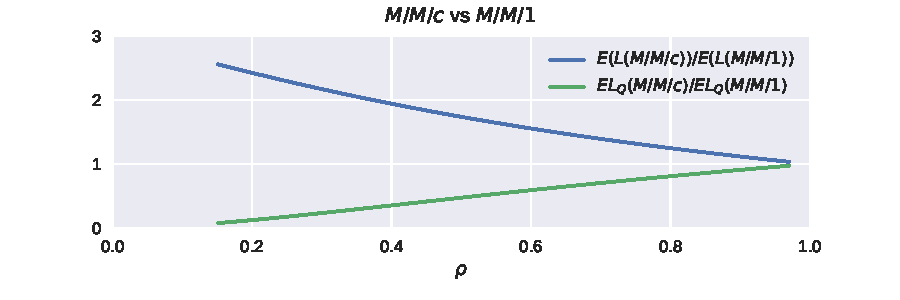
\includegraphics{multi_vs_single}
  \caption{multi server versus single fast server; here the number of
    servers $c=3$. We plot the ratio of the average number of jobs in
    the $M/M/3$ case and the $M/M/1$ queue with a fast server. (Note
    that by Little's law, the ratio between the waiting times is the
    same.) Clearly, jobs spend, on average, less time in queue in the
    $M/M/c$ case, but more time in total. This is as expected. In
    particular, if $\rho$ is small, the time in the system must be
    dominated by the service time. Since the average service time is
    three times as short at the fast server, the total time in the
    system must be approximately three times as long in the $M/M/3$
    case for $\rho$ is small. On the other hand, when $\rho$ is large,
    the queues are long, and the total time in the system is dominated
    by the queueing times.  As queued jobs depart from the queue at
    rate $3$, in both queueing systems, the average queueing times
    must be roughly equal. This we can also see clearly in the graph,}
  \label{fig:multisingle}
\end{figure}

Here is the code I used to make the graphs.

<<wrap=False,include=False,fig=False>>=
from math import exp, factorial
import matplotlib.pylab as plt
import seaborn as sns
sns.set_context("paper")


def G(labda, mu, c):
    rho = labda / mu / c
    res = sum((c * rho)**n / factorial(n) for n in range(c))
    res += (c * rho)**c / ((1 - rho) * factorial(c))
    return res


def ELQ(labda, mu, c):
    rho = labda / mu / c
    g = G(labda, mu, c)
    return (c * rho)**c / (factorial(c) * g) * rho / (1 - rho)**2


def ELS(labda, mu, c):
    rho = labda / mu / c
    return rho * c


def EL(labda, mu, c):
    return ELS(labda, mu, c) + ELQ(labda, mu, c)


labda = 10
mu = 11

c = 3

R = range(5, c * mu)
Q = []
L = []
load = []
for labda in R:
    Q.append(ELQ(labda, mu, c) / ELQ(labda, c * mu, 1))
    L.append(EL(labda, mu, c) / EL(labda, c * mu, 1))
    load.append(labda / mu / c)

plt.figure(figsize=(6, 2))
plt.subplot(111)
plt.axis([0, 1, 0, 3])
plt.title("$M/M/c$ vs $M/M/1$")
plt.plot(load, L, label="$E(L(M/M/c))/E(L(M/M/1))$")
plt.plot(load, Q, label="$EL_Q(M/M/c)/EL_Q(M/M/1)$")
plt.xlabel("$\\rho$")
plt.legend()
plt.subplots_adjust(bottom=0.24)

# plt.show()
filename = "figures/multi_vs_single.pdf"
plt.savefig(filename)
plt.close()
@

The reader should observe that this code is not particularly
efficient, many of the computations are done a few times. With
recursion quite a number of shortcuts can be made.

    \end{enumerate}
\end{solution}
\end{question}


%%% Local Variables:
%%% mode: latex
%%% TeX-master: "book"
%%% End:
